% ##################################################################################################################
\section{Trondheim}
\label{sec:trondheim}
\hfill \textbf{Authors:} Stefan Flügel, Julia Kern, Frederik Bockemühl

% ##################################################################################################################
The Institute of Transport Economics (TØI) has, in cooperation with Julia Kern from TU-Berlin and Frederik Bockemühl from Hasselts University, built a first prototype model for the region of Trondheim \citep[][]{FluegelKern_unpub_WTS_2014}.

The road network data was imported from a publicly accessible data base (Elveg). Figure~\ref{fig:trondheimnetwork} illustrates the network. 
%
\createfigure%
{Network and simulated traffic in Trondheim and surroundings}%
{Network and simulated traffic in Trondheim and surroundings for 6:55\,am \citep[source][]{FluegelEtAl_Samferdsel_2014}}%
{\label{fig:trondheimnetwork}}%
{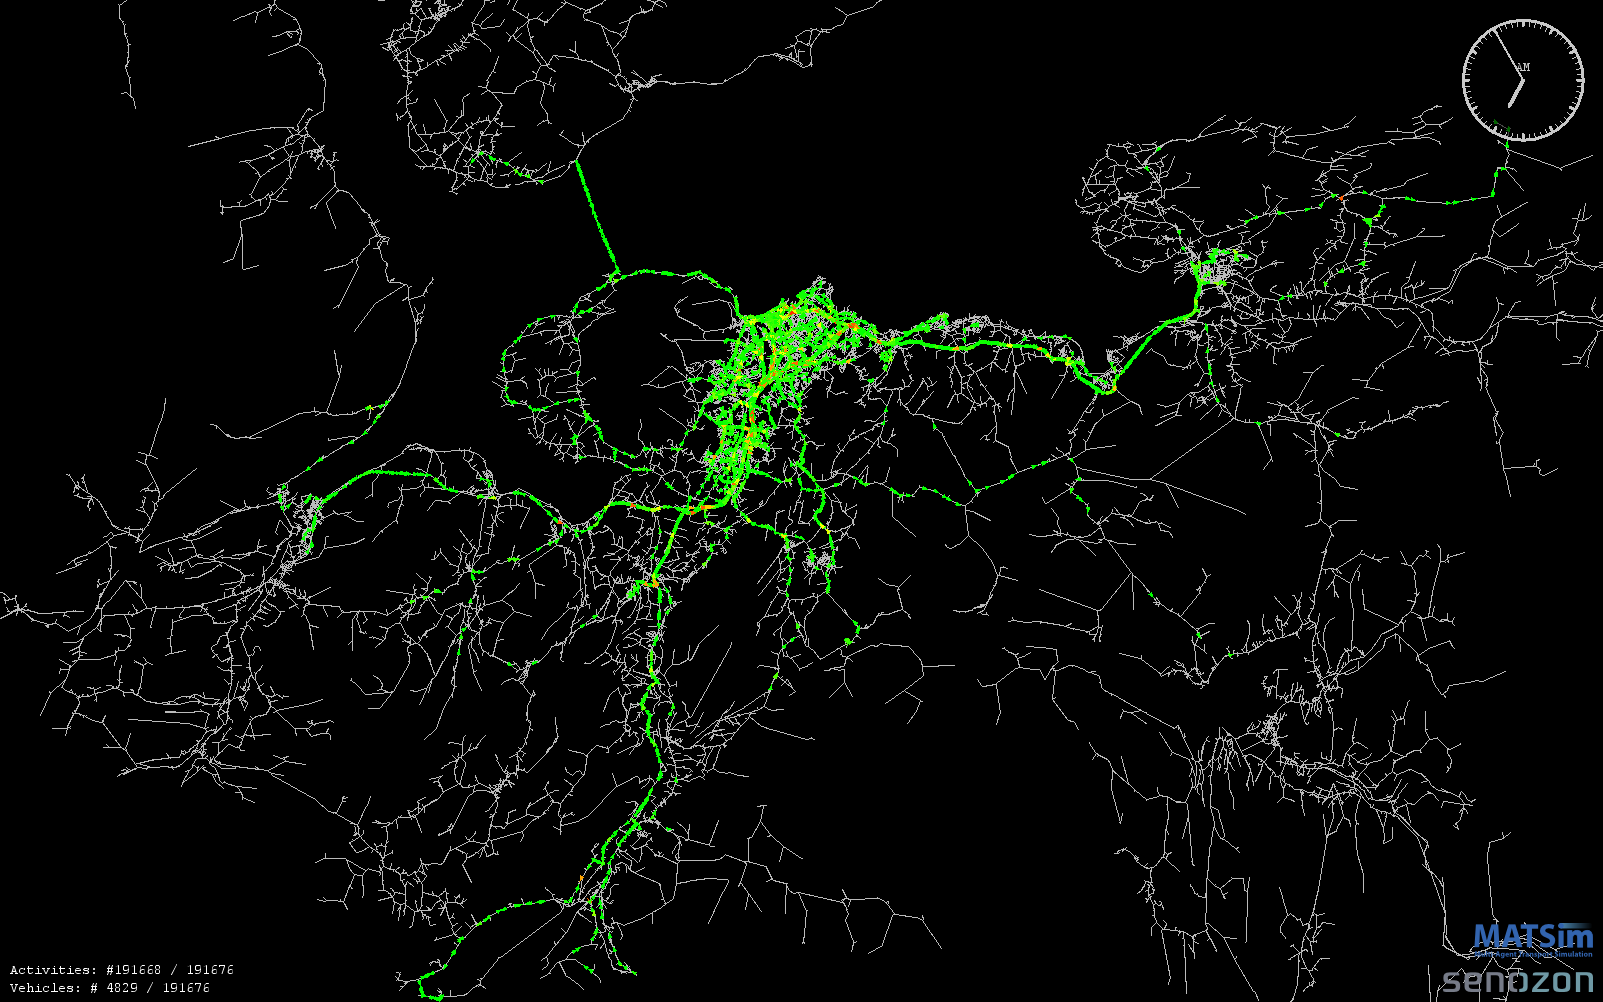
\includegraphics[width=0.85\textwidth, angle=0]{./using/figures/trondheimnetwork.png}}%
{}
%
Most required link information could directly be inferred from the data base. The lane capacity (vehicles per hour) was assumed to be a flat 1\,800 per lane. Existing toll stations with their current toll structures were coded manually in the network file. The public transport network is not implemented yet. The same applies to walk and cycle networks. Agents that take one of these modes were \gls{teleported} with travel times being calculated with predefined speeds per transport mode. 
The initial demand was derived from the travel diaries from the National Travel Survey (NTS 2009). 4\'453 respondents are simply scaled up to 191\,676 agents; activity locations and departure times were randomized a bit to avoid clusters. The current model differentiates only between work and "other" activities. Desirable working hours were specified to be 8\,hours. The demand consists only of private cars (no trucks). 

Standard utility functions were applied but in the calibration process, the default values for disutility from travel times in different transport modes were adjusted such that the model would reproduce the observed market shares. The fit of simulated traffic (in the reference scenario) against real-world counts was deemed satisfactory for the purpose of a first implementation \citep[][]{Bockemuehl_TechRep_UH_2014}. 

The standard behavioral modules in \gls{matsim} were included in the Trondheim model. That is, agent could react to policy measures by three choice dimensions: changing route, changing transport mode and changing departure time. To test if \gls{matsim} predicts reasonable behavioral changes, a small case study was performed. Additional tolls on streets (bridges and tunnels) to Trondheim city center were coded in the network and three congestion price structure were tested. Figure~\ref{fig:loadcurve} illustrates the effects on the simulated cars entering and leaving Trondheim city center. 
%
\createfigure%
{Cars entering/leaving Trondheim city center}%
{Cars entering/leaving Trondheim city center in reference scenario and three congestion pricing scenarios \citep[source][]{Bockemuehl_TechRep_UH_2014}}%
{\label{fig:loadcurve}}%
{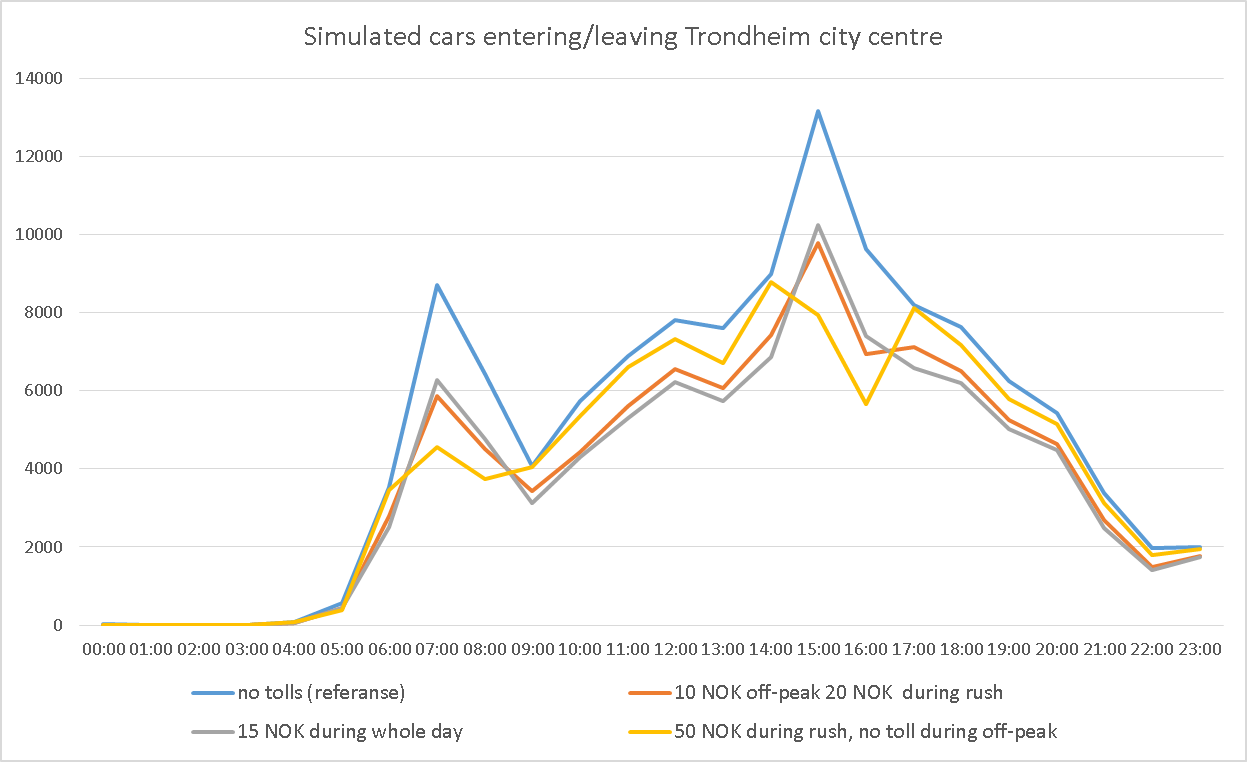
\includegraphics[width=0.85\textwidth, angle=0]{./using/figures/trondheimloadcurve.png}}%
{}
%
Compared to the reference scenario without tolls, the total number of cars was reduced in all toll scenarios. Some agents changed transport modes and some agents that would otherwise have driven through Trondheim center, changed their route. Comparing the three different congestion-pricing structures, it was also evident that agents changed departure time. The difference between the 15\,\gls{nok} flat scenario and the 10/20\,\gls{nok} scenario is small while the effect in the 50\,\gls{nok} rush scenario is substantial. Actually, in this scenario traffic was higher before 3\,pm and after 5\,pm implying that many agents changed departure time to avoid high congestion pricing.  

% ##################################################################################################################   










